\subsubsection*{Ziel}
Das Ziel ist  die Bestimmung der Parameter $K_{rk}$, $T_{nk}$  und $T_{vk}$ in
der Gleichung:

\begin{equation} \label{eq:pid:target}
    H_{rpid} = K_{rk} \cdot \biggl[ \frac{(1 + s \cdot T_{nk}) \cdot (1 + s \cdot T_{vk}) }{ s \cdot T_{nk} } \biggr]
\end{equation}


\subsubsection{Bestimmung der Reglerfrequenz $\omega_{pid}$}

Analog  zum PI-Regler  wird zuerst  im  Phasengang der  Strecke die  Frequenz
$\omega_{pid}$ bestimmt, f\"ur  welche die Phase der  Strecke einen bestimmten
Wert aufweist, nur wird hier $-135\degree$ benutzt:

\begin{equation} \label{eq:pid:phi_s}
    \varphi_s(\omega_{pid}) = -135 \degree
\end{equation}

In unserem Beispiel ergibt dies:

\begin{equation} \label{eq:pid:omega_pid}
    \omega_{pid} = \SI{0.6714}{\per\second}
\end{equation}


\subsubsection{Steigung des Phasengangs bei der Reglerfrequenz}

Anschliessend wird  die Steigung des  Phasengangs $\varphi_s$ der  Strecke bei
der  Frequenz  $\omega_{pid}$  bestimmt. Ausgangspunkt  daf\"ur  ist  die  von
\code{p\_sani} bestimmte  \"Ubertragungsfunktion der Strecke  (siehe Gleichung
\ref{eq:transfer:plant}).

\begin{equation} \label{eq:transfer:plant:derivative}
    \frac{d\varphi_s}{d\omega} \biggr \rvert_{\omega=\omega_{pid}}
        = \frac{d(arg(H_s(j\omega)))}{d\omega} \biggr \rvert_{\omega=\omega_{pid}}
        = \SI{-1.5124}{\second}
\end{equation}
\todo{Einheit \"uberpr\"ufen}


\subsubsection{Hilfsparameter $\beta$}

Zwischen den Steigungen der Phasen des offenen Regelkreises ($\varphi_o$), der
Strecke ($\varphi_s$) und des Reglers ($\varphi_r$) gilt folgende Beziehung:

\begin{equation} \label{eq:pid:phi_sum}
    \varphi_o = \varphi_s + \varphi_r
\end{equation}

Da die Ableitung eine lineare Funktion ist, gilt somit auch: \todo{korrekte Begriffe}
\begin{equation} \label{eq:pid:dphi_sum}
    \frac{d\varphi_o}{d\omega} = \frac{d\varphi_s}{d\omega} + \frac{d\varphi_r}{d\omega}
\end{equation}

Diese Beziehungen  k\"onnen auch  gut in Abbildung  \ref{fig:pid_complete} von
Hand \"uberpr\"uft werden.

Es soll nun gelten:

\begin{equation} \label{eq:pid:dphi_o_target}
    \frac{d\varphi_o}{d\omega} \biggr \rvert_{\omega=\omega_{pid}} = - \frac{1}{2}
\end{equation}

Da   $\frac{d\varphi_s}{d\omega}$  durch   die  Strecke   gegeben  und   somit
unver\"anderlich ist, kann lediglich der Wert von $\frac{d\varphi_r}{d\omega}$
angepasst     werden,     damit     $\frac{d\varphi_o}{d\omega}$     Gleichung
\ref{eq:pid:dphi_o_target} erf\"ullt.

Dazu f\"uhrt man den Hilfsparameter $\beta$ ein, f\"ur den gilt:

\begin{gather} \label{eq:pid:beta:start}
    \begin{split}
        \frac{1}{T_{vk}} & = \frac{\omega_{pid}}{\beta} \\
        \frac{1}{T_{nk}} & = \omega_{pid} \cdot \beta  \\
                       0 & <  \beta \leq 1
    \end{split}
\end{gather}

Die  beiden Frequenzen  $\frac{1}{T_{vk}}$  und  $\frac{1}{T_{nk}}$ sind  also
symmetrisch  um den  Faktor $\beta$  gr\"osser bzw.  kleiner als  die Frequenz
$\omega_{pid}$. \todo{siehe Plot} Will man  $\beta$ von Hand bestimmen, trifft
man zuerst eine ``vern\"unftige'' Annahme, zum Beispiel:

\begin{equation} \label{eq:pid:beta:initial_value}
    \beta = 0.5
\end{equation}

Mit  diesem Startwert  bestimmt  man nun  $T_{nk}$  und ${T_{vk}}$. Die  somit
erhaltenen Werte setzt man in  Gleichung \ref{eq:pid:target} ein, zusammen mit
dem Wert f\"ur $\omega_{pid}$ aus Gleichung \ref{eq:pid:omega_pid}:

\begin{gather} \label{eq:pid:t_nk_t_vk_initial_results}
    \begin{split}
        {T_{vk}} & = \frac{\beta}{\omega_{pid}}  = \frac{0.5}{\SI{0.6714}{\per\second}}                   = \SI{0.7447}{\second} \\
        {T_{nk}} & = \frac{1}{\omega_{pid} \cdot \beta} = \frac{1}{\SI{0.6714}{\per\second} \cdot 0.5 }  = \SI{2.9789}{\second} \\
    \end{split}
\end{gather}

Eingesetzt in die Reglergleichung, vorerst mit $K_{rk} = 1$:

\begin{gather} \label{eq:pid:t_nk_t_vk_initial_results}
    \begin{split}
        H_{rpid} & = K_{rk} \cdot \biggl[ \frac{(1 + j\omega \cdot T_{nk}) \cdot (1 + j\omega \cdot T_{vk}) }{ j\omega \cdot T_{nk} } \biggr] \\
                 & = 1      \cdot \biggl[ \frac{(1 + j\omega \cdot \SI{2.9789}{\second}) \cdot (1 + j\omega \cdot \SI{0.7447}{\second}) }{ j\omega \cdot  \SI{2.9789}{\second}} \biggr]
    \end{split}
\end{gather}

Von dieser Gleichung bestimmt man nun den Phasengang und wertet danach dessen
Ableitung an der Stelle $\omega = \omega_{pid}$ aus:

\begin{gather} \label{eq:pid:phi_r_first_iteration}
    \begin{split}
        \varphi_s (j\omega)                                            & = arg(H_{rpid}(j\omega))        \\
        \frac{d\varphi_s}{d\omega} \biggr \rvert_{\omega=\omega_{pid}} & = \SI{1.1920}{\second}
    \end{split}
\end{gather}
\todo{Die zugeh\"orige Rechnung ist lange und m\"uhsam, allenfalls in Anhang? Ebenfalls: Einheit kontrollieren}


Setzt man dies in Gleichung \ref{eq:pid:phi_sum} ein, erh\"alt man:
\begin{gather} \label{eq:pid:phi_sum_result_iteration_one}
    \begin{split}
    \frac{d\varphi_o}{d\omega}       \biggr \rvert_{\omega=\omega_{pid}, \beta=0.5}
        & = \frac{d\varphi_s}{d\omega} \biggr \rvert_{\omega=\omega_{pid}}
        + \frac{d\varphi_r}{d\omega} \biggr \rvert_{\omega=\omega_{pid}, \beta=0.5} \\
        & = \SI{-1.5124}{\second} + \SI{1.1920}{\second} \\
        & = \SI{-0.3204}{\second} \\
        & > -\frac{1}{2}
    \end{split}
\end{gather}

Mit  $\beta  = 0.5$  erh\"alt  man  also eine  zu  hohe  Steigung des  offenen
Regelkreises   an    der   Stelle  $\omega_{pid}$,   folglich   muss   $\beta$
{\em{verkleinert}} werden.   Diese Berechnungen  werden nun mit  jeweils neuen
Werten  f\"ur  $\beta$  solange  wiederholt,  bis  die  Steigung  des  offenen
Regelkreises die gew\"unschte N\"ahe zu $-\frac{1}{2}$ aufweist.

Da die manuelle Iterierung dieses Prozesses enorm viel Zeit in Anspruch nimmt,
bietet  sich  hier  eine  Automatisierung  an. Die  Berechnung  mittels  eines
geeigneten Algorithmus in Matlab liefert schlussendlich folgendes Ergebnis:
\todo{Allenfalls Matlab-Algo in Anhang und Verweis}

\begin{gather} \label{eq:pid:beta_result}
    \begin{split}
        \beta    & = 0.2776 \\
        {T_{vk}} & = \frac{\beta}{\omega_{pid}}           = \SI{0.4134}{\second} \\
        {T_{nk}} & = \frac{1}{\omega_{pid} \cdot \beta}   = \SI{5.3656}{\second} \\
    \end{split}
\end{gather}

Sollte  man  f\"ur  $\beta$  einen komplexen  Wert  erhalten,  wird  $\beta=1$
gesetzt.\todo{Wie kann dies egtl. passieren?}


\subsubsection{Durchtrittsfrequenz $\omega_d$}

Diese  Werte setzt man nun in Gleichung \ref{eq:pid:target} ein. $K_{rk}$ wird
wie bei der Bestimmung von $\beta$ vorerst noch auf 1 gesetzt.

\begin{gather} \label{eq:pid:h_rpid_beta_result}
    \begin{split}
        H_{rpid} & = K_{rk} \cdot \biggl[ \frac{(1 + s \cdot T_{nk}               ) \cdot (1 + s \cdot T_{vk}               ) }{ s \cdot T_{nk}               } \biggr]
                   = 1      \cdot \biggl[ \frac{(1 + s \cdot \SI{5.3656}{\second} ) \cdot (1 + s \cdot \SI{0.4134}{\second} ) }{ s \cdot \SI{5.3656}{\second} } \biggr]
    \end{split}
\end{gather}

Zur Bestimmung von $K_{rk}$ wird nun der Frequenzgang des offenen Regelkreises
betrachtet. Dazu  multipliziert  man  wie  gehabt  die  \"Ubertragungsfunktion
der  Strecke   (siehe  Gleichung   \ref{eq:transfer:plant})  mit   der  soeben
bestimmten  provisorischen   \"Ubertragungsfunktion  des   Reglers  (Gleichung
\ref{eq:pid:h_rpid_beta_result}).

\begin{equation} \label{eq:pid:h_o_k_rk_one}
    H_{o}(j\omega) = H_{rpid}(j\omega) \cdot H_s(j\omega)
\end{equation}

Nun wird  die Durchtrittsfrequenz $\omega_d$  bestimmt, an welcher  der offene
Regelkreis eine  Verst\"arkung von $\SI{0}{\decibel} =  1$ aufweisen soll. Wie
auch  beim  PI-Regler  werden  wir   hier  ein  \"Uberschwingen  von  $16.3\%$
anstreben, womit gem\"ass Tabelle \ref{tab:phi_s}gilt:

\begin{equation} \label{eq:pid:omega_d_target}
    \varphi_s(\omega_d) = \varphi_s = -128.5\degree
\end{equation}

Dieser Wert wird analog zum PI-Regler aus dem Phasengang des offenen Regelkreises
abgelesen. \todo{siehe Plot} Eine Nachrechnung mittels Matlab ergibt:


\begin{equation} \label{eq:pid:omega_d_target}
    \omega_d = \SI{0.5341}{\per\second}
\end{equation}


\subsubsection{Bestimmung der Reglerverst\"arkung $K_{rk}$}

In einem letzten Schritt wird  nun der Amplitudengang des offenen Regelkreises
an der  Stelle $\omega_d$ gleich 1  gesetzt und diese Gleichung  nach $K_{rk}$
aufgel\"ost:

\begin{equation} \label{eq:pid:h_o_k_rk_one}
    \begin{split}
        A_{o}(j\omega_d)    & = | H_{o}(j\omega_d) |                            \\
                            & = | H_{rpid}(j\omega_d) \cdot H_s(j\omega_d) |    \\
                            & = \Biggl \rvert
                                    K_{rk}
                                    \cdot
                                    \biggl[ \frac{(1 + j\omega_d \cdot T_{nk}) \cdot (1 + j\omega_d \cdot T_{vk}) }{ j\omega_d \cdot T_{nk} } \biggr] \Biggr \rvert \\
                            & \cdot
                                \Biggl \rvert
                                    K_s
                                    \cdot \frac{1}{1 + j\omega_d \cdot T_1}
                                    \cdot \frac{1}{1 + j\omega_d \cdot T_2}
                                    \cdot \frac{1}{1 + j\omega_d \cdot T_2}
                                    \Biggr \rvert \\
                            & = 1
    \end{split}
\end{equation}

Mit den gegebenen und berechneten Werten:
\begin{gather} \label{eq:pid:h_o_k_rk_one}
    \begin{split}
        K_s         & = 2                        \\
        T_1         & = \SI{0.4134}{\second}     \\
        T_2         & = \SI{1.4894}{\second}     \\
        T_3         & = \SI{5.3655}{\second}     \\
        T_{nk}      & = \SI{5.3656}{\second}     \\
        T_{vk}      & = \SI{0.4134}{\second}     \\
        \omega_d    & = \SI{0.5341}{\per\second}
    \end{split}
\end{gather}

Dies liefert:

\begin{equation} \label{eq:pid:k_rk_result}
    K_{rk} = 1.83084
\end{equation}


\subsubsection{Resultat}

Somit ist der Regler vollst\"andig bestimmt und hat folgende \"Ubertragungsfunktion:

\begin{equation} \label{eq:pid:result}
    H_{rpid}(s) = 1.83084 \cdot \biggl[ \frac{(1 + s \cdot \SI{5.3656}{\second} ) \cdot (1 + s \cdot \SI{0.4134}{\second} ) }{ s \cdot \SI{5.3656}{\second} } \biggr]
\end{equation}

Die Frequenzg\"ange der Strecke, des Reglers und des offenen Regelkreises:

\begin{figure}[h! width=\pagewidth]
    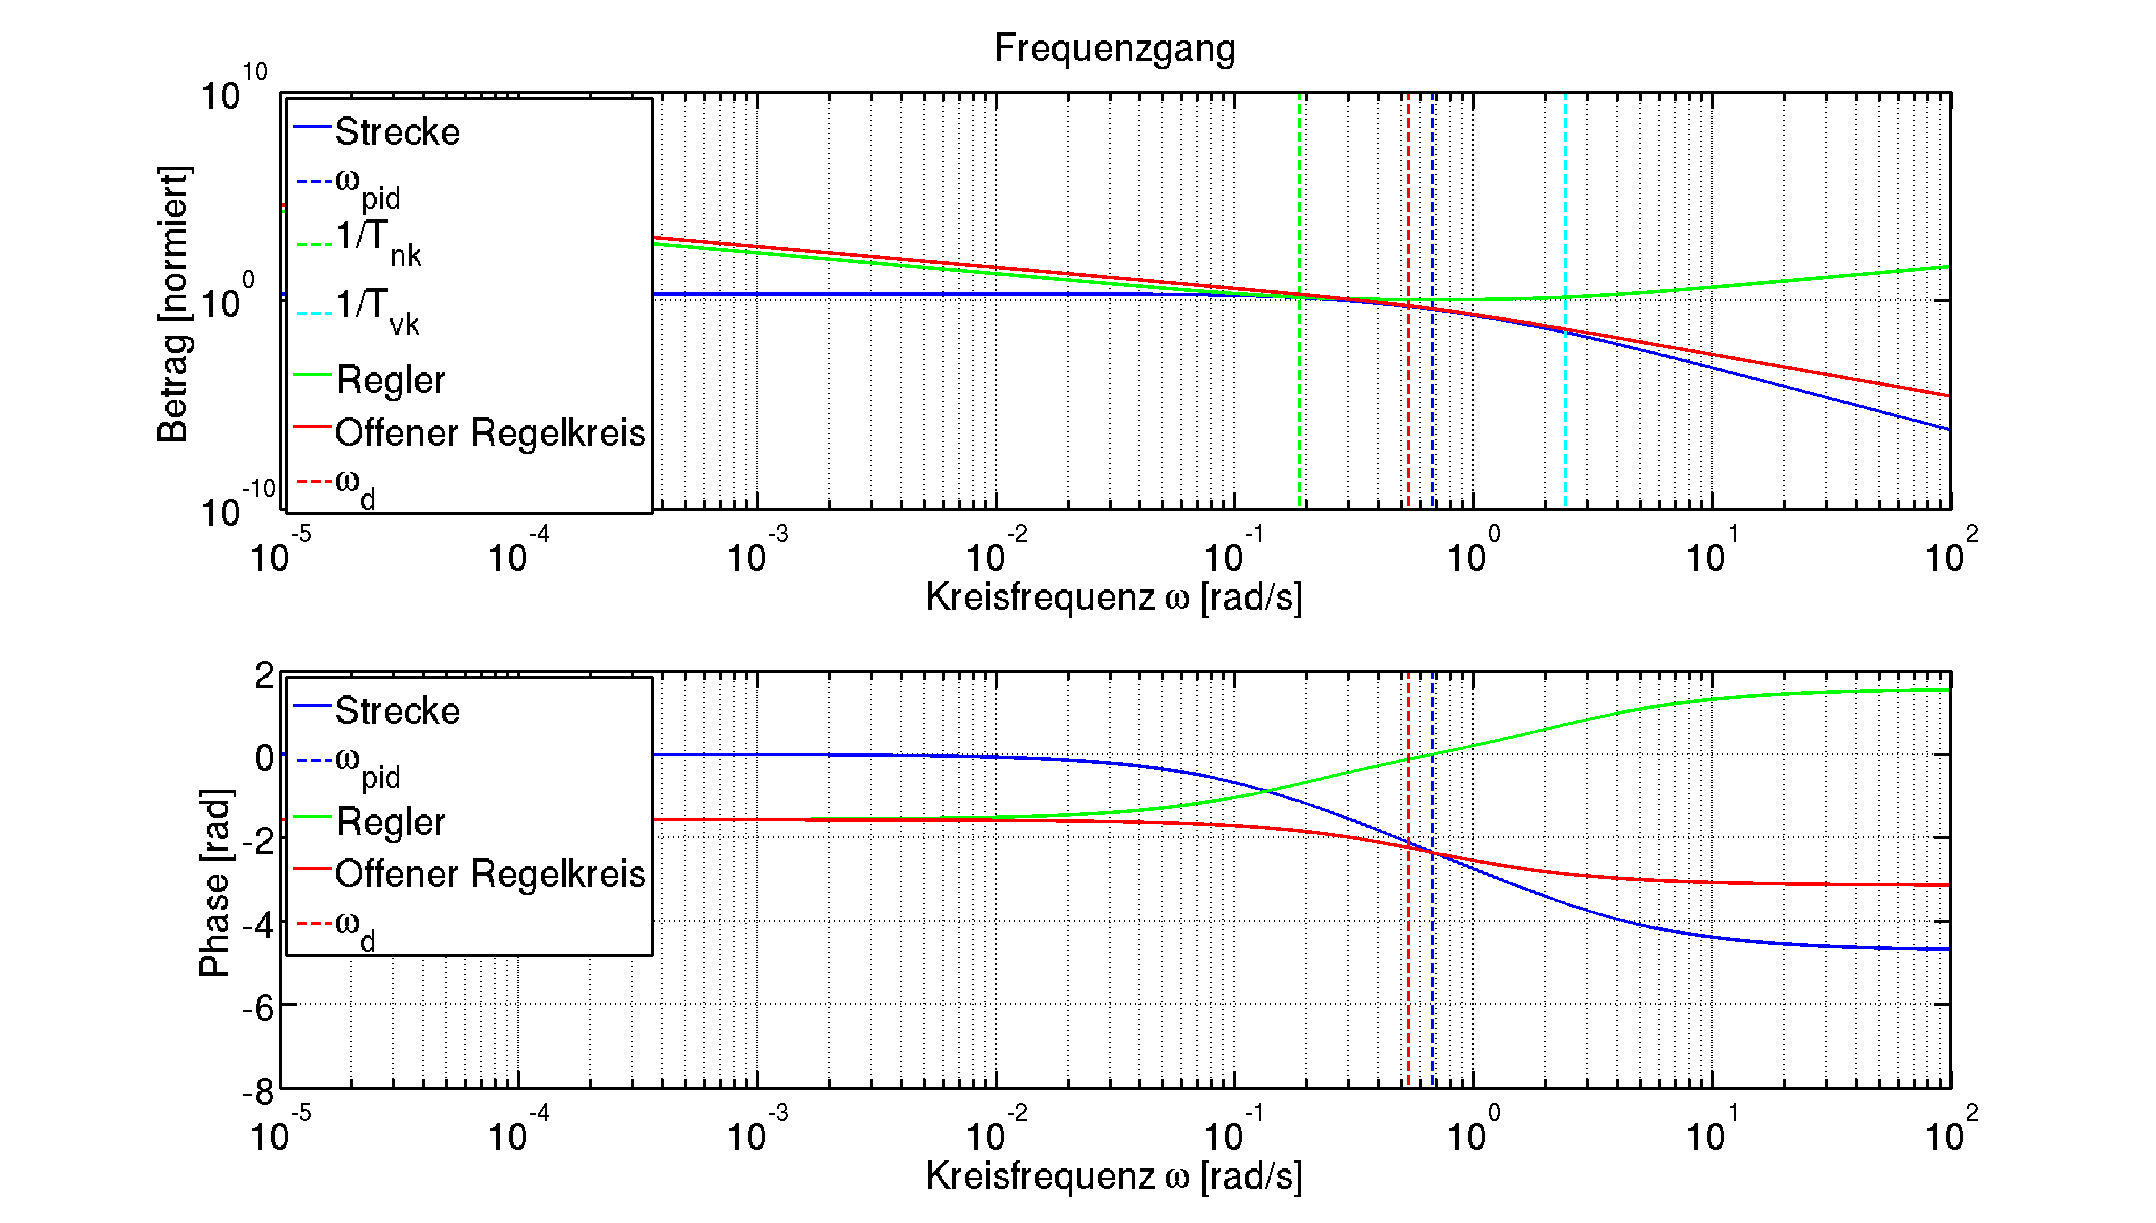
\includegraphics[width=\textwidth]{images/pidCompletePlot.png}
    \caption{%
        Frequenzgang der Strecke (blau), des  Reglers (gr\"un) und des offenen
        Regelkreises  (rot).  Ebenfalls  eingetragen  sind die  Reglerfrequenz
        $\omega_{pid}$,   die   beiden   Frequenzen   $\frac{1}{T_{vk}}$   und
        $\frac{1}{T_{nk}}$ sowie die Durchtrittsfrequenz $\omega_d$.
    }
    \label{fig:pid_complete}
\end{figure}
\clearpage
